\chapter{Propuesta}\label{chapter:proposal}

En el presente capítulo se presenta la metodología empleada para la predicción de los resultados de las diferentes eventos del atletismo en importantes competencias. Se expone el estudio realizado sobre el conjunto de datos necesarios, la modelación de las marcas de los atletas, la idea detrás del algoritmo de predicción y, por último, el proceso de optimización para escoger el valor de algunos parámetros importantes que influyen en las predicciones finales sin necesidad de contar con criterios de experto. 

\section{Concepción general de la solución}

En este trabajo se propone una metodología que permita predecir la posición que ocuparán los atletas en el ranking final de cada uno de los eventos de una competencia de atletismo. Para esto, se concibe la estructura general del proceso de predicción con las siguientes etapas: captura de los datos de una fuente fiable, preprocesamiento y limpieza de los datos, modelado de una función de los resultados para cada atleta y, por último, la ejecución de simulaciones junto con un estudio estadístico de los resultados para brindar una propuesta final de pronóstico para cada evento. (Figura \ref{fig:diagram1})

\begin{figure}[H]
    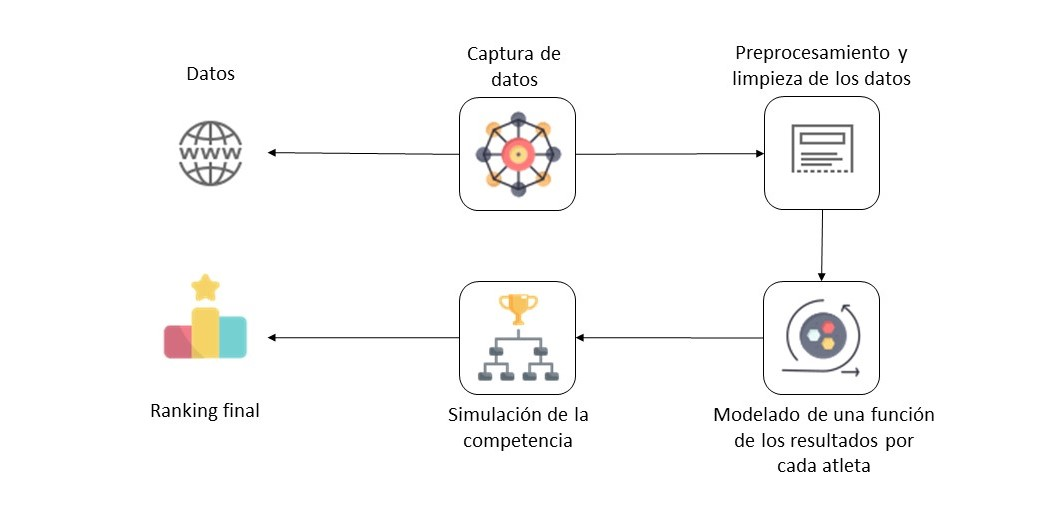
\includegraphics[width=\linewidth]{Graphics/diagram1.jpg}
    \caption{Pipeline de la metodología propuesta para la predicción del ranking final de los diferentes eventos que conforman una competencia de atletismo}
    \label{fig:diagram1}
\end{figure}

\subsection{Captura y preprocesamiento de los datos}

El sistema de predicción que se propone se basa únicamente en resultados obtenidos por los atletas en competencias pasadas para la construcción del ranking más probable de cada evento. Por esta razón, en un primer momento, es primordial definir cuáles son los datos con los que se va a trabajar.

Para una competencia en específico, se requiere conocer los datos expuestos a continuación: 

\begin{itemize}
    \item El nombre de la competencia.
    \item La fecha de inicio de la competencia, importante para la validación de las marcas de los atletas, ya que se desea ser lo más transparente y justo posible en el proceso de predicción y no tomar marcas posteriores al comienzo de la competencia.
    \item Las disciplinas que forman parte de la competencia y sus modalidades (masculino y femenino); es necesario conocerlas todas, puesto que cada una se analizará de manera individual.
    \item Para cada disciplina, si el objetivo de los atletas es obtener la mayor o menor marca, dato importante para la construcción de los rankings.
    \item La lista de nombres de los atletas que se presentarán en cada una de las modalidades.
    \item De cada atleta su nombre, país al que representa y las marcas obtenidas en un número determinado de competencias previas, importante para la construcción de la función de sus resultados.
\end{itemize}

\subsection{Modelado de la función de resultados de un atleta}

Como se ha podido comprobar en la bibliografía consultada en el capítulo anterior, la creación de modelos capaces de obtener posibles resultados futuros de los atletas y consecuentes con sus actitudes pasadas se ha atacado desde varias perspectivas. Muchos se han basado en diferentes datos recopilados, como es el caso de las marcas personales obtenidas, velocidades máximas alcanzadas en el caso de las carreras de velocidad y variables relacionadas con el metabolismo y con las características fisiológicas de los atletas.

El objetivo de esta investigación es poder construir un modelo que solo cuente con las marcas personales de los atletas para la predicción de futuros resultados. Una idea es encontrar una variable aleatoria que pueda describir los resultados de un atleta en un evento en particular y en un tiempo dado. Para que esta variable sea capaz de generar resultados nuevos, es importante encontrar primero una distribución de probabilidad que la caracterice. Una alternativa posible para encontrar esta distribución es modelarla a partir de métodos de estimación de densidad.

Los métodos de estimación de densidad son herramientas estadísticas que se utilizan para reconstruir o estimar una función de densidad de probabilidad (PDF) desconocida a partir de un conjunto de muestras extraídas. Estos estimadores se clasifican en paramétricos y no paramétricos. Un estimador no paramétrico no utiliza suposiciones a priori sobre la distribución subyacente para obtener estimaciones sobre esta distribución. En comparación, un estimador paramétrico asume la forma funcional de la PDF subyacente y utiliza las muestras u observaciones para obtener estimaciones de los parámetros que definen la forma de la PDF. Un ejemplo de un estimador paramétrico sería asumir que la forma de la PDF que se estima es gaussiana y usar las muestras para obtener estimaciones de la media y la desviación estándar de la distribución gaussiana. Los estimadores no paramétricos no hacen suposiciones sobre la forma de la distribución y, por lo tanto, son herramientas más flexibles para capturar distribuciones donde no se conoce información suficiente a priori \cite{burke2016kernel}.

Uno de los estimadores no paramétricos más empleados es la Estimación de la Densidad del Kernel (KDE) \cite{rosenblatt1956remarks}. Dado un valor  $x_i$  la función aprendida por KDE devuelve la densidad de la distribución en el punto  $x_i$ . Esta densidad, cuyo valor está acotado al rango $[0, + \infty )$, es una medida relativa de verosimilitud (likelihood). Si la densidad para el punto A es mayor que la de B, significa que la probabilidad de que A pertenezca a la distribución es mayor que la de B. Esta técnica permite crear una curva suave dado un conjunto de datos aleatorios. La estimación también se puede usar para generar puntos que solo parecen provenir de un conjunto de muestras específico. Esta característica es particularmente útil en el presente trabajo y la razón principal por la que KDE fue escogida.

La definición formal de KDE, dado un conjunto de muestras $ X_1, \cdots, X_n $ de una PDF subyacente, es: 

\begin{equation}
    \label{eq:kde}
    \hat{p_n} (x) = \frac{1}{nh} \sum_{i=1}^{n} K (\frac{X_i - x}{h})
\end{equation}
 
donde $K(x)$ se denomina función kernel, que define la forma y la distribución de la influencia (peso) que se asocian a cada observación y $h > 0$ se denomina ancho de banda, que controla la cantidad de suavizado (cuánto se expande la influencia de cada observación). Básicamente, el KDE suaviza cada punto de datos $X_i$ en pequeñas protuberancias de densidad y, luego, suma todas estas pequeñas protuberancias para obtener la estimación de densidad final.

El ancho de banda $h$ es un parámetro fundamental a la hora de utilizar KDE. Si el ancho de banda es muy pequeño reproduce detalles de los datos que son insignificantes y se adjudican a ruido estadístico debido a que es una cantidad de muestras finita. Por otro lado, si el ancho de banda es muy grande se genera un sobre-suavizado que puede hacer que se pierdan de vista algunas características de la distribución. Por lo tanto, la elección de un ancho de banda se trata de una relación de compromiso entre no reproducir ruido estadístico y una buena descripción de la distribución. 

Luego de definir formalmente a KDE y hacer un análisis de sus características y las ventajas que posee, es seleccionado para la modelación de la función de resultados de cada atleta. La función de kernel escogida para definir la forma y la distribución de la influencia que se asocian a cada observación es la gaussiana. Por otro lado, el análisis de los datos para escoger el mejor valor de ancho de banda a menudo se ha realizado mediante un enfoque de prueba y error. Si se pudiera acordar un método eficiente que, usando los datos, permitiera determinar de forma automática este valor, la utilidad de KDE mejoraría enormemente. La vía propuesta para escoger este valor se explica en la sección \ref{sec:params_opt}.

En aras de poder construir el mejor modelo que represente al atleta en el momento de la competencia, se hace uso solo de marcas obtenidas en una cantidad específica de años anteriores al momento que se desea predecir. Además, se realiza un trabajo de preprocesamiento con el vector de resultados para cada atleta, mediante una ponderación de los años escogidos, donde se les asigna un mayor peso a los años más recientes. De esta forma, si la competencia se lleva a cabo en el año 2022 y se toman $n$ años, solo se escogen las marcas de los años $ 2022,\ 2021, \cdots,\ 2022 - (n-1)$ y a cada año se le asigna un peso $w$. Por tanto, para el entrenamiento del modelo se le pasan las marcas del año 2022 repetidas $w_{2022}$ veces, las del año 2021 aparecerán $w_{2021}$ veces y así en adelante. 

Uno de los problemas que puede aparecer una vez se analizan los datos extraídos es que existe una gran ambigüedad en aquellos casos de atletas con muy pocas marcas registradas. Puede existir el caso de que un atleta tenga una sola marca muy buena registrada, pero solo haberla obtenido en una ocasión, lo cual no se puede considerar muy confiable. Es por esto que se propone agregar, además, un parámetro \textit{alpha} que modifique las marcas de la siguiente manera:

\begin{equation}
    \label{eqn:alpha1}
    pondVal = (1 + \frac{alpha}{cantMarcas}) 
\end{equation}
\begin{equation}
    \label{eqn:alpha2}
    marca_i = marca_i * pondVal
\end{equation}

Esto permite premiar a aquellos atletas que cuentan con un mayor número de marcas, ya que en ese caso es más confiable el hecho de que se repitan. De esta forma, mientras menos marcas tiene un atleta mayor será el valor resultante de cada marca (para eventos donde se busca maximizar el valor de la marca se toma \textit{alpha} negativo).

Una vez ya se tienen definidos los parámetros de KDE y las marcas preprocesadas de los atletas, se pasa a construir la función de densidad de probabilidad de cada uno con la fórmula \ref{eq:kde}. De esta forma, ya de cada variable aleatoria de los atletas se conoce su distribución, por lo que es posible generar resultados nuevos. 

\subsection{Simulación de la competencia}\label{sec:met_sim}

Una vez analizada la técnica a utilizar para modelar los posibles resultados de un atleta a partir de las marcas obtenidas anteriormente, se pasa a la modelación de una competencia específica de atletismo. Para ello, cada evento de la competencia se analiza por separado y se obtiene una predicción del ranking final. El algoritmo se mantiene igual para cada uno, pero varían los valores de los parámetros presentados en la sección anterior para la modelación de la función de los resultados de los atletas. Además, se añade uno nuevo, que es la cantidad de simulaciones a realizar. 

El algoritmo de predicción de un evento en específico cuenta con las siguientes etapas:

En un primer momento, se construyen los modelos KDE de los resultados de todos los atletas siguiendo el procedimiento explicado en la sección anterior. Una vez obtenidos, ya es posible generar nuevas marcas acordes con las obtenidas en otras competencias y que se usaron para la construcción del modelo.

Luego, por cada atleta en la lista de participantes, se produce una marca nueva y se construye un ranking, organizándolos de menor a mayor en caso de que el objetivo del evento sea obtener la marca más pequeña, y de mayor a menor en caso contrario. Finalmente, este experimento se repite un número $n$ de veces y se obtienen $n$ rankings, a partir de los cuales se construye la propuesta final con las primeras 8 posiciones.

Existen varias vías para la construcción del ranking final. Una primera idea es para cada posición, colocar el atleta que más se repita sin contar los que hayan sido ya escogidos para ocupar posiciones anteriores. Pero en este caso, no se le da prioridad a un atleta que no es el que más se repite en una posición $i$ pero si en las anteriores y aún no ha sido escogido.

Es por esto que se le realiza una modificación a idea anterior. Esta vez, se trata de encontrar para cada posición $i$ del ranking final el atleta que más queda como primero en los $n$ rankings obtenidos, eliminando de cada uno  aquellos atletas que ya hayan sido escogidos para ocupar posiciones anteriores.

\section{Optimización de parámetros}\label{sec:params_opt}

En el apartado anterior se pudo observar que el algoritmo propuesto depende de ciertos parámetros cuyo valor debe ser escogido cuidadosamente, puesto que influyen directamente en la calidad de los resultados obtenidos. Estos son: el ancho de banda de los modelos KDE de los atletas, el valor de \textit{alpha} con el cual se trata de crear un balance entre los atletas que tienen pocas marcas registradas contra los que tienen muchas, la ponderación que va a tener cada año, la cantidad de años a utilizar y, por último, el número de simulaciones a realizar.

\subsection{Metodología}

La selección de estos valores se decidió hacerla por evento y no por competencia, ya que se considera que cada evento tiene su propio comportamiento y sus propias peculiaridades, por lo que es mejor analizarlos por separado. De esta forma, para todos los atletas pertenecientes a una misma modalidad (evento y sexo), su modelo se construirá de forma equivalente. El número de simulaciones a ejecutar para realizar el experimento también es independiente en cada evento. 

La idea detrás del proceso de optimización propuesto consiste en hacer un análisis de una competencia ya celebrada en el pasado y cuyos resultados finales son conocidos. Para cada evento se genera un conjunto de configuraciones, donde cada configuración está conformada por un valor asignado a cada parámetro de interés. Luego, con cada una de estas configuraciones se ejecuta el proceso de simulación explicado en la sección \ref{sec:met_sim}. Este proporciona una propuesta de ranking final, cuyo error debe ser calculado con respecto al ranking real conocido. Quedan aún dos cuestiones por resolver: ¿cómo se calcula el error del ranking propuesto con respecto al real?, y ¿cómo se genera el espacio de configuración para cada evento?

\subsection{Cálculo de error}\label{sec:errors}

Un paso importante durante el proceso de optimización es el cálculo de cuan buena es una predicción con respecto al resultado real. Para esto se cuenta con las primeras ocho posiciones del ranking real y con todas las posiciones de los atletas dentro del ranking obtenido luego de la simulación. Se proponen dos ideas para el cálculo de este error.

\begin{itemize}
    \item Error 1: la suma de las diferencias para cada atleta de la posición que ocupa dentro del ranking final con la posición que ocupa en el ranking predicho.
    \item Error 2: se presenta un enfoque diferente y se tratan los rankings como un sistema de recomendación. Los atletas son tratados como documentos y aquellos que hayan quedado en las primeras posiciones del ranking real son considerados ``relevantes'', mientras que los demás ``no relevantes''. A los atletas ``relevantes'' se le asigna un ranking igual a ocho menos la posición que ocupan, para los no ``relevantes'' el ranking es cero. Al realizar esta modelación se aprovecha de los estudios ya realizados para estos sistemas y se utiliza el error \textit{ndcg score}. Este error fue considerado debido a que no solo se quiere conocer acerca de los atletas que quedaron en las ocho primeras posiciones (recuperados) sino también que tan lejos estuvieron y este error lo toma en cuenta.
\end{itemize}

\subsection{Generación del espacio de configuración}

El ajuste de hiperparámetros, a veces denominado optimización de hiperparámetros (HPO), es el proceso que trata de aprovechar al máximo un modelo al identificar la mejor configuración para él con respecto a la métrica que se haya elegido. 

El problema de configuración del algoritmo se puede formular formalmente de la siguiente manera: dado un algoritmo parametrizado A (el algoritmo objetivo), un conjunto (o distribución) de instancias del problema I y una métrica de costo c, encuentre la configuración del parámetro de A que minimice c en I. La métrica de costo c a menudo se basa en el tiempo de ejecución requerido para resolver una instancia de problema o, en el caso de problemas de optimización, en la calidad de la solución lograda dentro de un tiempo previamente fijado \cite{hutter2011sequential}.

El aprendizaje automático automatizado (AutoML), es el proceso de automatizar las tareas lentas e iterativas del desarrollo de modelos de aprendizaje automático (ML). Permite que los desarrolladores, analistas y científicos de datos creen modelos de aprendizaje automático con un escalado, eficiencia y productividad altos, al mismo tiempo que mantiene la calidad del modelo. Uno de los subproblemas de AutoML es ofrecer la mejor instancia de modelo posible de todos los algoritmos disponibles. Cada uno de estos algoritmos es ajustable mediante hiperparámetros, entradas al algoritmo que modifican su comportamiento. 

En el presente trabajo se propone el uso de las herramientas AutoML en la optimización de hiperparámetros. Existen principalmente dos razones por las cuales se decidió usarlas. Primero, encontrar el mejor parámetro a mano es una tarea bastante tediosa y la combinatoria del espacio de configuración puede ser bastante grande. Segundo, no hay absolutamente ninguna garantía de que la configuración escogida para un conjunto de datos determinado funcione tan bien para otro. Por lo que, cada vez que se aplica el modelo a un nuevo conjunto de datos, es crucial refinar los hiperparámetros. 

Una opción podría ser usar la fuerza bruta, pero el espacio de configuraciones puede ser enorme. La búsqueda aleatoria es otra opción, pero no existe garantía de converger a la mejor configuración, al menos en un período de tiempo determinado. El uso de tecnologías AutoML permite abordar estas dos limitaciones mediante la automatización de la exploración del espacio de configuración.

Los parámetros constituyen un componente fundamental de la metodología de predicción propuesta. En un primer momento, los valores de estos pueden ser ajustados si se cuenta con expertos en el tema que puedan evaluar cuan buenas son las predicciones e ir ajustando el modelo en busca de mejoras. Sin embargo, se propone el desarrollo de un optimizador capaz de realizar el proceso de selección de los valores de forma automática. En el próximo capítulo se da paso a una primera implementación del prototipo, capaz de poner a prueba la metodología planteada a través de un proceso de experimentación y análisis de los resultados. 